\documentclass[11pt]{article}
\usepackage[margin=1.5in]{geometry}
\usepackage{graphicx}
\usepackage{float}
\usepackage{parskip}
\usepackage{amsmath}
\usepackage{subfigure}
\usepackage{ulem}
\usepackage{pgfplots}
\pgfplotsset{width=10cm, compat=1.9}

\begin{document}

\textbf{\Huge Trigonometric Identities and \\ Equations}

Athan Zhang \& Jeffrey Chen

\section{Law of Sines and Cosines}
By now, students know how to solve right triangles using trigonometric ratios. The Law of Sines and Cosines will allow students to solve \textbf{oblique triangles} or non-right triangles. 

\subsection{Law of Sines}
The \textbf{Law of Sines} states the following:

\begin{center}
If $\triangle ABC$ has side lengths $a$, $b$, and $c$ corresponding to opposite angles $\angle A$, $\angle B$, and $\angle C$, then $\frac{\sin(A)}{a} = \frac{\sin(B)}{B} = \frac{\sin(C)}{c}$.
\end{center}
This law is helpful in cases where you are given the measures of two angles and a nonincluded side (AAS), two angles and the included side (ASA), or two sides and a nonincluded angle (SSA).

\subsection{Law of Cosines}
The \textbf{Law of Cosines} states the following:
\begin{center}
If $\triangle ABC$ has side lengths $a$, $b$, and $c$ corresponding to opposite angles $\angle A$, $\angle B$, and $\angle C$, then $c^2 = a^2 + b^2 - 2ab\cos C$.
\end{center}
This law is helpful in cases when you are given the measures of three sides of a triangle (SSS) or when you are given two sides and their included angle (SAS).

\section{Area of a Triangle}
Besides the typical formula $A = \frac{1}{2}bh$ to calculate the area of a triangle, which may prove cumbersome to find the height of a triangle, there are other alternatives to find the area of a triangle using only their side lengths and angles.

\subsection{Area of Triangle Given SAS}
Let's consider a triangle with side lengths $a$ and $b$, and the included angle between these sides denoted by $\theta$ (measured in radians). Our goal is to determine the area $A$ of this triangle.

We know that $b\sin(\theta)$ gives us the altitude, a length that will be perpendicular to $a$. We can then use that in the area of a triangle formula. Substituting the given values into the formula, we obtain:

\begin{equation*}
A = \frac{1}{2}ab\sin(\theta)
\end{equation*}

\subsection{Heron's Formula}
Consider a triangle with side lengths $a$, $b$, and $c$, and let $s$ be the semiperimeter of the triangle, defined as $s = \frac{1}{2}(a + b + c)$. Heron's formula states that the area $A$ of the triangle can be calculated using the following formula:

\begin{equation*}
A = \sqrt{s(s - a)(s - b)(s - c)}
\end{equation*}

\section{Basic Identities}

\subsection{Reciprocal and Quotient Identities}

Reciprocal and quotient identities are essential relationships between trigonometric functions that provide alternative ways to express these functions in terms of their reciprocals or as ratios of other trigonometric functions. Understanding these identities is crucial for simplifying trigonometric expressions and solving trigonometric equations. The following table showcases these identities.

\begin{table}[H]
    \centering
    \begin{tabular}{|c c c|c|}
    \hline
         & Reciprocal Identities & & Quotient Identities \\
         \hline
         &&&\\
        $\displaystyle \sin\theta = \frac{1}{\csc\theta}$ &  $\displaystyle \cos\theta = \frac{1}{\sec\theta}$ & $\displaystyle \tan\theta = \frac{1}{\cot\theta}$ & $\displaystyle \tan\theta = \frac{\sin\theta}{\cos\theta}$ \\ &&&\\
        $\displaystyle \csc\theta = \frac{1}{\sin\theta}$ &  $\displaystyle \sec\theta = \frac{1}{\cos\theta}$ & $\displaystyle \cot\theta = \frac{1}{\tan\theta}$ & $\displaystyle \cot\theta = \frac{\cos\theta}{\sin\theta}$ \\
        &&&\\
    \hline
    \end{tabular}
\end{table}

\subsection{Pythagorean Identities}
The Pythagorean identities are a set of fundamental equations in trigonometry that are derived from the Pythagorean theorem. These identities establish relationships between the trigonometric functions of an angle in a right triangle.

\begin{table}[H]
    \centering
    \begin{tabular}{|c c c|}
    \hline
    & Pythagorean Identities & \\
    \hline
    &&\\
        $\displaystyle \sin^2\theta + \cos^2\theta = 1$\hspace{1cm} &  $\displaystyle \tan^2\theta + 1 = \sec^2\theta$\hspace{1cm} & $\displaystyle \cot^2\theta + 1 = \csc^2\theta$ \\
    &&\\
    \hline
    \end{tabular}
\end{table}

\subsection{Cofunction Identities}
Another set of basic trigonometric identities involves cofunctions. A trigonometric cofunction exists when two trigonometric functions $f$ and $g$ satisfy $f(\alpha) = g(\beta)$ where $\alpha$ and $\beta$ are complementary angles in a right triangle.

\begin{table}[H]
    \centering
    \begin{tabular}{|ccc|}
    \hline
         & Cofunction Identities &  \\
         \hline
         &&\\
        $\displaystyle \sin\theta = \cos\left(\frac{\pi}{2} - \theta\right)$ & $\displaystyle \tan\theta = \cot\left(\frac{\pi}{2} - \theta\right)$ & $\displaystyle \sec\theta = \csc\left(\frac{\pi}{2} - \theta\right)$ \\
         &&\\
        $\displaystyle \cos\theta = \sin\left(\frac{\pi}{2} - \theta\right)$ & $\displaystyle \cot\theta = \tan\left(\frac{\pi}{2} - \theta\right)$ & $\displaystyle \csc\theta = \sec\left(\frac{\pi}{2} - \theta\right)$ \\
         &&\\
        \hline
    \end{tabular}

\end{table}

\subsection{Odd-Even Identities}
Odd-even identities are a set of trigonometric identities that relate the behavior of trigonometric functions with respect to the sign of the angle. These identities are based on the observation that some trigonometric functions are odd while others are even functions.


\begin{table}[H]
    \centering
    \begin{tabular}{|ccc|}
    \hline
         & Odd-Even Identities & \\
         \hline
         &&\\
        $\displaystyle \sin(-\theta) = -\sin\theta$ & $\displaystyle \cos(-\theta) = \cos\theta$ & $\displaystyle \tan(-\theta) = -\tan\theta$ \\
         &&\\
        $\displaystyle \csc(-\theta) = -\csc\theta$ & $\displaystyle \sec(-\theta) = \sec\theta$ & $\displaystyle \cot(-\theta) = -\cot\theta$ \\
         &&\\
    \hline
    \end{tabular}
\end{table}

\section{Sum and Difference Identities}
The sum and difference identities deal with trigonometric functions of the sum or difference of two variables. These are often useful when the angle inside a cosine or sine function can be written as the sum or difference of special angles.

Let's consider two angles, $\alpha$ and $\beta$. The distance $d$ in the following two unit circles is equal. 
\begin{figure}[H]
    \centering
    \includegraphics[width=0.8\textwidth]{Precalc/images/sumdiffdiagram.jpg}
\end{figure}
Through the first unit circle, we can use the distance formula to find that
\begin{align*}
    d^2 = (\cos\alpha - \cos\beta)^2 + (\sin\alpha - \sin\beta)^2
\end{align*}
And from the second unit circle, we find that
\begin{align*}
    d^2 = (\cos(\alpha-\beta) - 1)^2 + (\sin(\alpha-\beta) - 0)^2
\end{align*}
We can set these two expression equal to each other, giving us
{\scriptsize  
    \begin{align*}
        (\cos\alpha - \cos\beta)^2 + (\sin\alpha - \sin\beta)^2 &= (\cos(\alpha-\beta) - 1)^2 + (\sin(\alpha-\beta) - 0)^2 \\
        \cos^2\alpha - 2\cos\alpha\cos\beta + \cos^2\beta + \sin^2\alpha - 2\sin\alpha\sin\beta + \sin^2\beta &= \cos^2(\alpha-\beta) - 2\cos(\alpha-\beta) + 1 + \sin^2(\alpha-\beta) \\
        (\cos^2\alpha + \sin^2\alpha) - 2(\cos\alpha\cos\beta + \sin\alpha\sin\beta) + (\cos^2\beta + \sin^2\beta) &= (\cos^2(\alpha-\beta) + \sin^2(\alpha-\beta)) - 2\cos(\alpha-\beta) + 1 \\
        2 - 2(\cos\alpha\cos\beta + \sin\alpha\sin\beta) &= 2 - 2\cos(\alpha-\beta) \\
        \cos\alpha\cos\beta + \sin\alpha\sin\beta &= \cos(\alpha-\beta)
    \end{align*}
}%
Giving us the final identity of
\begin{align*}
    \cos(\alpha-\beta) = \cos\alpha\cos\beta + \sin\alpha\sin\beta
\end{align*}
Using the Cofunction and Odd-Even identities, we are further able to manipulate this identity to get the other sum and difference identities.

By replacing $\beta$ with $-\beta$, we get
\begin{align*}
    \cos(\alpha-(-\beta)) &= \cos\alpha\cos(-\beta) + \sin\alpha\sin(-\beta) \\
    \cos(\alpha+\beta) &= \cos\alpha\cos\beta - \sin\alpha\sin\beta \\
\end{align*}
By replacing $\alpha$ with $\frac{\pi}{2} - \alpha$, we get
\begin{align*}
    \cos\left(\frac{\pi}{2} - \alpha + \beta\right) &= \cos\left(\frac{\pi}{2} - \alpha\right)\cos\beta - \sin\left(\frac{\pi}{2} - \alpha\right)\sin\beta \\
    \cos\left(\frac{\pi}{2} - (\alpha - \beta)\right) &= \sin\alpha\cos\beta - \cos\alpha\sin\beta \\ 
    \sin(\alpha-\beta)  &= \sin\alpha\cos\beta - \cos\alpha\sin\beta \\
\end{align*}
And then again, by replacing $\beta$ with $-\beta$, we get
\begin{align*}
    \sin(\alpha-(-\beta)) &= \sin\alpha\cos(-\beta) - \cos\alpha\sin(-\beta) \\
    \sin(\alpha+\beta) &= \sin\alpha\sin\beta + \cos\alpha\cos\beta \\
\end{align*}
We can also divide these identities, giving us
\begin{align*}
    \tan(\alpha - \beta) &= \frac{\sin(\alpha-\beta)}{\cos(\alpha-\beta)} \\
    &= \frac{\sin\alpha\cos\beta - \cos\alpha\sin\beta}{\cos\alpha\cos\beta + \sin\alpha\sin\beta} \\
    &= \frac{\sin\alpha\cos\beta - \cos\alpha\sin\beta}{\cos\alpha\cos\beta(1 + \tan\alpha\tan\beta)} \\
    &= \frac{\tan\alpha - \tan\beta}{1 + \tan\alpha\tan\beta}
\end{align*}
Finally, once again substituting $\beta$ with $-\beta$, we get
\begin{align*}
    \tan(\alpha-(-\beta)) &= \frac{\tan\alpha - \tan(-\beta)}{1 + \tan\alpha\tan(-\beta)} \\
    \tan(\alpha+\beta) &=  \frac{\tan\alpha + \tan\beta}{1 - \tan\alpha\tan\beta} \\
\end{align*}
A table of all the Sum and Difference Identities can be seen below.
\begin{table}[H]
    \centering
    \begin{tabular}{|c|c|}
    \hline
         Sum Identities & Difference Identities \\
         \hline
         &\\
        $\displaystyle \cos(\alpha+\beta) = \cos\alpha\cos\beta - \sin\alpha\sin\beta$ & $\displaystyle \cos(\alpha-\beta) = \cos\alpha\cos\beta + \sin\alpha\sin\beta$
        \\ &\\
        $\displaystyle \sin(\alpha+\beta) = \sin\alpha\cos\beta + \cos\alpha\sin\beta$  & $\displaystyle \sin(\alpha-\beta) = \sin\alpha\cos\beta - \cos\alpha\sin\beta$  
        \\ &\\
        $\displaystyle \tan(\alpha+\beta) = \frac{\tan\alpha + \tan\beta}{1-\tan\alpha\tan\beta}$ & $\displaystyle \tan(\alpha-\beta) = \frac{\tan\alpha - \tan\beta}{1+\tan\alpha\tan\beta}$ \\&\\
    \hline
    \end{tabular}
\end{table}

\section{Multiple-Angle Identities}


\subsection{Double Angle}
Using the sum identities and setting $\phi$ equal to $\theta$, we can derive the following double-angle identities:

\begin{table}[H]
    \centering
    \begin{tabular}{|c c c|}
    \hline
         & Double-Angle Identities &\\
         \hline
         &&\\
        $\displaystyle \sin2\theta = 2\sin\theta\cos\theta$\hspace{1cm} & $\displaystyle \cos2\theta = \cos^2\theta-\sin^2\theta$\hspace{1cm} & $\displaystyle \tan2\theta = \frac{2\tan\theta}{1-\tan^2\theta}$ \\
        &&\\
    \hline
    \end{tabular}
\end{table}

\subsection{Power-Reducing Identities}
By rearranging the equation for the cosine double-angle identity, we can obtain an identity for the value of $\sin^2x$. This can be useful when we want to reduce the power of trigonometric functions.

For example,
\begin{align*}
    \cos 2\theta &= \cos^2\theta - \sin^2\theta \\
    \sin^2 \theta &= \cos^2 \theta - \cos 2\theta \\
    \sin^2 \theta &= (1 - \sin^2 \theta) - \cos 2\theta \\
    2\sin^2 \theta &= 1 - \cos 2\theta \\
    \sin^2 \theta &= \frac{1 - \cos 2\theta}{2} \\
\end{align*}
Additionally,
\begin{align*}
    \cos 2\theta &= \cos^2\theta - \sin^2\theta \\
    \cos^2 \theta &= \cos 2\theta + \sin^2\theta \\ 
    \cos^2 \theta &= \cos 2\theta + (1 - \cos^2 \theta) \\
    2\cos^2 \theta &= \cos 2\theta + 1 \\
    \cos^2 \theta &= \frac{1 + \cos 2\theta}{2} \\
\end{align*}
Finally,
\begin{align*}
    \tan^2 \theta &= \frac{\sin^2 \theta}{\cos^2 \theta} \\
    &= \frac{1 - \cos 2\theta}{1 + \cos 2\theta}
\end{align*}

The table below summarizes these identities.
\begin{table}[H]
    \centering
    \begin{tabular}{|c c c|}
    \hline
     & Power-Reducing Identities & \\
     \hline
         &&\\
        $\displaystyle \sin^2\theta = \frac{1-\cos2\theta}{2}$\hspace{1cm} & $\displaystyle \cos^2\theta = \frac{1+\cos2\theta}{2}$\hspace{1cm}& $\displaystyle \tan^2\theta = \frac{1-\cos2\theta}{1+\cos2\theta}$\\
         &&\\
    \hline
    \end{tabular}
\end{table}

\subsection{Half Angle}
The half-angle identities serve a similar function to the double-angle identities. They can be easily derived from the Power-Reducing identities by setting $\theta = \frac{1}{2}\theta$.
\begin{align*}
    \sin^2{\frac{\theta}{2}} &= \frac{1 - \cos{2(\frac{\theta}{2}})}{2} \\
    \sin^2{\frac{\theta}{2}} &= \frac{1 - \cos{\theta}}{2} \\
    \sin{\frac{\theta}{2}} &= \pm\sqrt{\frac{1 - \cos\theta}{2}} \\
\end{align*}
and
\begin{align*}
    \cos^2{\frac{\theta}{2}} &= \frac{1 + \cos{2(\frac{\theta}{2})}}{2} \\
    \cos^2{\frac{\theta}{2}} &= \frac{1 + \cos\theta}{2} \\
    \cos{\frac{\theta}{2}} &= \pm\sqrt{\frac{1 + \cos\theta}{2}}
\end{align*}
and finally
\begin{align*}
    \tan^2{\frac{\theta}{2}} &= \frac{1 - \cos{(2\frac{\theta}{2})}}{1 + \cos{2(\frac{\theta}{2})}} \\
    \tan^2{\frac{\theta}{2}} &= \frac{1 - \cos\theta}{1 + \cos\theta} \\
    \tan{\frac{\theta}{2}} &= \sqrt{\frac{1 - \cos\theta}{1 + \cos\theta}} \\
    \tan{\frac{\theta}{2}} &= \sqrt{\frac{1 - \cos\theta}{1 + \cos\theta} \times \frac{1 + \cos\theta}{1 + \cos\theta}} \\
    \tan{\frac{\theta}{2}} &= \sqrt{\frac{\sin^2}{(1 + \cos\theta)^2}} \\
    \tan{\frac{\theta}{2}} &= \frac{\sin\theta}{1 + \cos\theta} \\
\end{align*}
Giving us the following identities:
\begin{table}[H]
    \centering
    \begin{tabular}{|c c c|}
    \hline
        & Half Angle Identities & \\
        \hline
        &&\\
        $\displaystyle \sin\left(\frac{\theta}{2}\right) = \pm \sqrt{\frac{1 - \cos(\theta)}{2}}$ & $\displaystyle \cos\left(\frac{\theta}{2}\right) = \pm \sqrt{\frac{1 + \cos(\theta)}{2}}$ & $\displaystyle \tan\left(\frac{\theta}{2}\right) = \frac{\sin(\theta)}{1 + \cos(\theta)}$\\
        &&\\ 
        \hline
    \end{tabular}

\end{table}

\section{Product-to-Sum Identities}
The product-to-sum identities allow us to rewrite products of trigonometric functions as sums instead. We can manipulate the sum and difference identities to get the Product to SUm Identities. They are listed below:

\begin{table}[H]
    \centering
    \begin{tabular}{|c c|}
    \hline
    \multicolumn{2}{|c|}{Product-to-Sum Identities} \\
    \hline
    &\\
    $\displaystyle \sin\alpha\sin\beta = \frac{1}{2} \left[ \cos(\alpha-\beta) - \cos(\alpha+\beta) \right] $ & $\sin\alpha\cos\beta = \frac{1}{2} \left[ \sin(\alpha-\beta) + \sin(\alpha+\beta) \right]$\\
    &\\
    $\displaystyle \cos\alpha\cos\beta = \frac{1}{2} \left[ \cos(\alpha-\beta) + \cos(\alpha+\beta) \right] $ & $\cos\alpha\sin\beta = \frac{1}{2} \left[ \sin(\alpha-\beta) - \sin(\alpha+\beta) \right]$ \\
    &\\
    \hline
    \end{tabular}
\end{table}

There are also corresponding Sum-to-Product identities:

\begin{table}[H]
    \centering
    \begin{tabular}{|c c|}
    \hline
        \multicolumn{2}{|c|}{Sum-to-Product Identities} \\
        \hline
        &\\
        $\sin\alpha + \sin\beta = 2\sin\left(\frac{{\alpha+\beta}}{2}\right)\cos\left(\frac{{\alpha-\beta}}{2}\right)$ & $\sin\alpha - \sin\beta = 2\cos\left(\frac{{\alpha+\beta}}{2}\right)\sin\left(\frac{{\alpha-\beta}}{2}\right)$ \\
        &\\
        $\cos\alpha + \cos\beta = 2\cos\left(\frac{{\alpha+\beta}}{2}\right)\cos\left(\frac{{\alpha-\beta}}{2}\right)$ & $\cos\alpha - \cos\beta = -2\sin\left(\frac{{\alpha+\beta}}{2}\right)\sin\left(\frac{{\alpha-\beta}}{2}\right)$ \\
        &\\
        \hline
    \end{tabular}
\end{table}

\section{Trigonometric Equations}
Solving trigonometric equations employs many of the same techniques as solving algebraic equations. However, we must consider whether the input variables apply to the trigonometric equation.

Since trigonometric functions are periodic, there are often infinite solutions to trigonometric equations. Take, for example, the equation $\cos x = \frac{1}{2}$

\begin{center}
    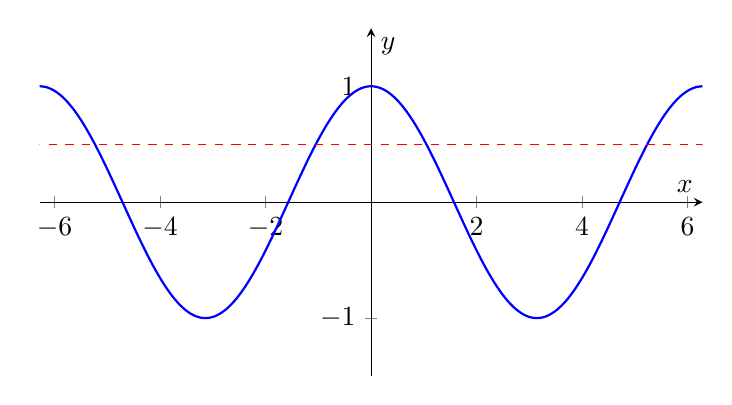
\begin{tikzpicture}
    \begin{axis}[
    xlabel=$x$,
    ylabel=$y$,
    xmin=-2*pi,
    xmax=2*pi,
    ymin=-1.5,
    ymax=1.5,
    domain=-2*pi:2*pi,
    samples=100,
    axis lines=middle, width=10cm, height=6cm,
    smooth]
      
    % Plotting the function cos(x)
    \addplot[blue, thick] {cos(deg(x))};
    
    % Plotting the line x = 1/2
    \addplot[red, dashed] coordinates {(-8, 0.5) (8, 0.5)};
    
    \end{axis}
    \end{tikzpicture}
\end{center}
We can see that there are two solutions in the domain [0, 2$\pi$), $x = \frac{\pi}{3}$ and $x = \frac{5\pi}{3}$. Since $y = \cos x$ has a period of $2\pi$, there are infinitely many solutions for $x$ in the domain ($-\infty$, $\infty$). We can then express a solution for $x$ as 
\begin{align*}
    x = \frac{\pi}{3} \pm 2\pi n & & \text{and} & & x = \frac{5\pi}{3} \pm 2\pi n
\end{align*}
Where $n$ is any integer.

To solve much more complex trigonometric identities, we must use our identities.

\subsection*{Example:}

Find all solutions of $2\cos^2{x} - \sin{x} = 1$ on the interval [0, $2\pi$).

\begin{align*}
    2\cos^2{x} - \sin{x} &= 1 & \text{Given} \\
    2\cos^2{x} - \sin{x} - 1 &= 0 & \text{Subtract 1 from both sides} \\
    2(1 - \sin^2{x}) - \sin{x} - 1 &= 0 & \text{Pythagorean Identity} \\
    2 - 2\sin^2{x} - \sin{x} - 1 &= 0 & \text{Distribute} \\
    -2\sin^2{x} - \sin{x} + 1 &= 0 & \text{Simplify} \\
    (-2\sin{x} + 1)(\sin{x} + 1) &= 0 & \text{Factor} \\
\end{align*}
We then have
\begin{align*}
    -2\sin{x} + 1 &= 0 \\
    \sin{x} &= \frac{1}{2} \\
    x &= \frac{\pi}{6}, \frac{5\pi}{6} \\
\end{align*}
and
\begin{align*}
    \sin{x} + 1 &= 0 \\
    \sin{x} &= - 1 \\
    x &= \frac{3\pi}{2} \\
\end{align*}



\end{document}